\section{Effort and cost estimation}

Organizations must generate estimates for both the effort and cost involved in software development. 
Two primary methodologies are commonly employed for this purpose:
\begin{itemize}
    \item \textit{Experience-based techniques}: this approach relies on the manager's experiences with similar projects and a deep understanding of the application domain.
        The manager draws upon their knowledge to make well-informed judgments regarding the likely effort requirements for future projects.
        In implementing this methodology, the following steps are essential:
        \begin{enumerate}
            \item Identify the deliverables to be generated in the new project, encompassing both documents and software.
            \item Record these deliverables systematically in a spreadsheet.
            \item Assess and estimate the effort required for each individual deliverable.
            \item Calculate the cumulative effort necessary for the entire project.
        \end{enumerate}
        It is generally beneficial to engage the entire team in the process of effort estimation and encourage each team member to articulate and justify their individual estimates.
    \item \textit{Algorithmic cost modeling:}: this method utilizes a formulaic approach to calculate project effort.
        Estimates are derived from assessments of product attributes (e.g., size) and process characteristics (e.g., the expertise of the staff involved).
        The formulaic model provides a structured and systematic way to determine the effort and cost associated with the software development project.
        The estimation process relies on a mathematical function involving product, project, and process attributes, with values determined by project managers:
        \[\text{Effort}=\text{A}\cdot\text{Size}\cdot\text{B}\cdot\text{M}\]
        Here, A represents an organization-dependent constant, Size quantifies the product's quantity, B accounts for the disproportionate effort in large projects, and M serves as a multiplier reflecting attributes related to product, process, and personnel.
        While most models share a similar structure, they may employ distinct values for A, B, and M.
\end{itemize}

\subsection{Size estimation accuracy}
The precise size of a software system can only be determined with certainty upon its completion.
The final size is influenced by various factors, including the use of COTS (Components Off The Shelf), programming language, and the team's distribution. 
As the development process advances, the size estimate becomes increasingly accurate. 
On the other haned, the assessments of the factors contributing to B and M are subjective, varying based on the judgment of the estimator.
The potential approaches include:
\begin{enumerate}
    \item Extract the primary characteristics of the software from the RASD or other informal preliminary documents, categorize them in terms of Function Points, and then determine the software Lines of Code (LOC) estimation based on the number of Function Points.
    \item Directly estimate the LOC using insights from prior experiences or projects.
\end{enumerate}
Regardless of the approach chosen, it is crucial to complement any estimation with a complexity analysis to identify projects with particularly intricate requirements.

\paragraph*{Function points}
The function points approach, introduced by Allan Albrecht in 1975 while at IBM, revolves around characterizing the size of software based on its functional capabilities. 
This method quantifies function points through an amalgamation of program characteristics, encompassing data structures, inputs and outputs, inquiries, and external interfaces.
Each element type in the function point count is assigned a weight. 
The total function points are computed by multiplying the raw count of each element type by its corresponding weight and summing up all partial values:
\[\text{FP}=\sum{\left(\text{number of elements of a given type}\right) \cdot \left(\text{type weight}\right)}\]
The function types are elucidated in the following diagram:
\begin{figure}[H]
    \centering
    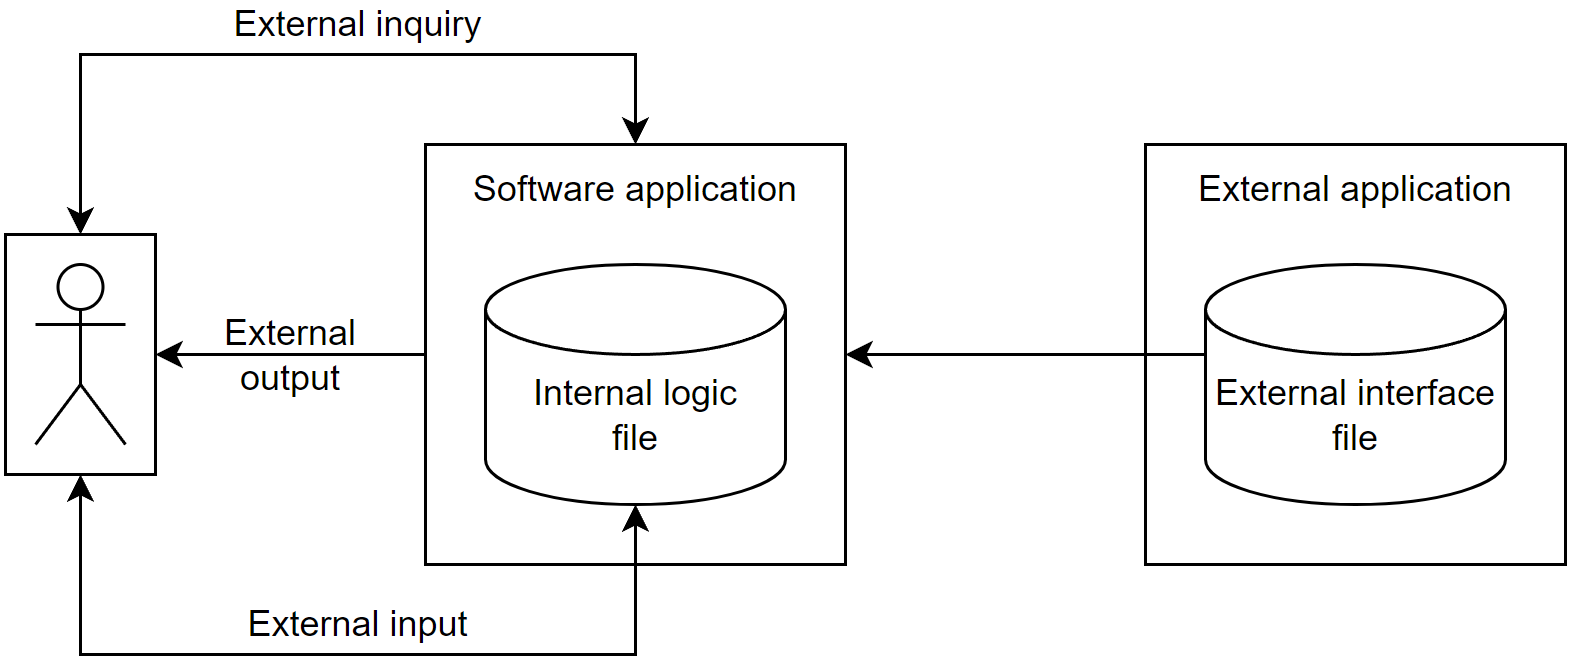
\includegraphics[width=0.75\linewidth]{images/ft.png}
\end{figure}
This classification results in the following function types:
\begin{itemize}
    \item \textit{Internal logic file} (ILF): homogeneous set of data used and managed by the application.
    \item \textit{External interface file} (EIF): homogeneous set of data used by the application but generated and maintained by other applications.
    \item \textit{External input}: elementary operation to process data from the external environment.
    \item \textit{External output}: elementary operation that produces data for the external environment, often involving the processing of data from logic files.
    \item \textit{External inquiry}: elementary operation that involves input and output without significant processing of data from logic files.
\end{itemize}
The function cost, determined by the assigned weights, can be visually represented in tabular format as depicted below:
\begin{table}[H]
    \centering
    \begin{tabular}{|c|ccc|}
    \hline
    \multirow{2}{*}{\textbf{Function types}} & \multicolumn{3}{c|}{\textbf{Weight}}                                                           \\ \cline{2-4} 
                                             & \multicolumn{1}{c|}{\textit{Simple}} & \multicolumn{1}{c|}{\textit{Medium}} & \textit{Complex} \\ \hline
    Inputs                                   & \multicolumn{1}{c|}{3}               & \multicolumn{1}{c|}{4}               & 6                \\
    Outputs                                  & \multicolumn{1}{c|}{4}               & \multicolumn{1}{c|}{5}               & 7                \\
    Inquiry                                  & \multicolumn{1}{c|}{3}               & \multicolumn{1}{c|}{4}               & 6                \\
    ILF                                      & \multicolumn{1}{c|}{7}               & \multicolumn{1}{c|}{10}              & 15               \\
    EIF                                      & \multicolumn{1}{c|}{5}               & \multicolumn{1}{c|}{7}               & 10               \\ \hline
    \end{tabular}
\end{table}
\begin{example}
    Consider the preceding function points weight table. 
    Calculate the function points (FP) for an application managing a mobile telephony service. 
    The application has the following characteristics:
    \begin{enumerate}
        \item Manages data about users and different types of rates, storing user data (phone number, personal information, rate type, applied promotions), with each rate type characterized by call cost, text message cost, and internet surfing cost. 
            Promotions modify specific cost items for a defined period.
        \item Enables users to access and modify their information, change rates, and activate promotions.
        \item Manages user billing based on data received from the network management system, covering voice calls (call duration, and the user location in case of roaming), SMS (the information that messages have been sent, and the corresponding user location in case of roaming), and internet (connection duration, amount of downloaded data, user location) of each user.
    \end{enumerate}
    The corresponding diagram is provided below:
    \begin{figure}[H]
        \centering
        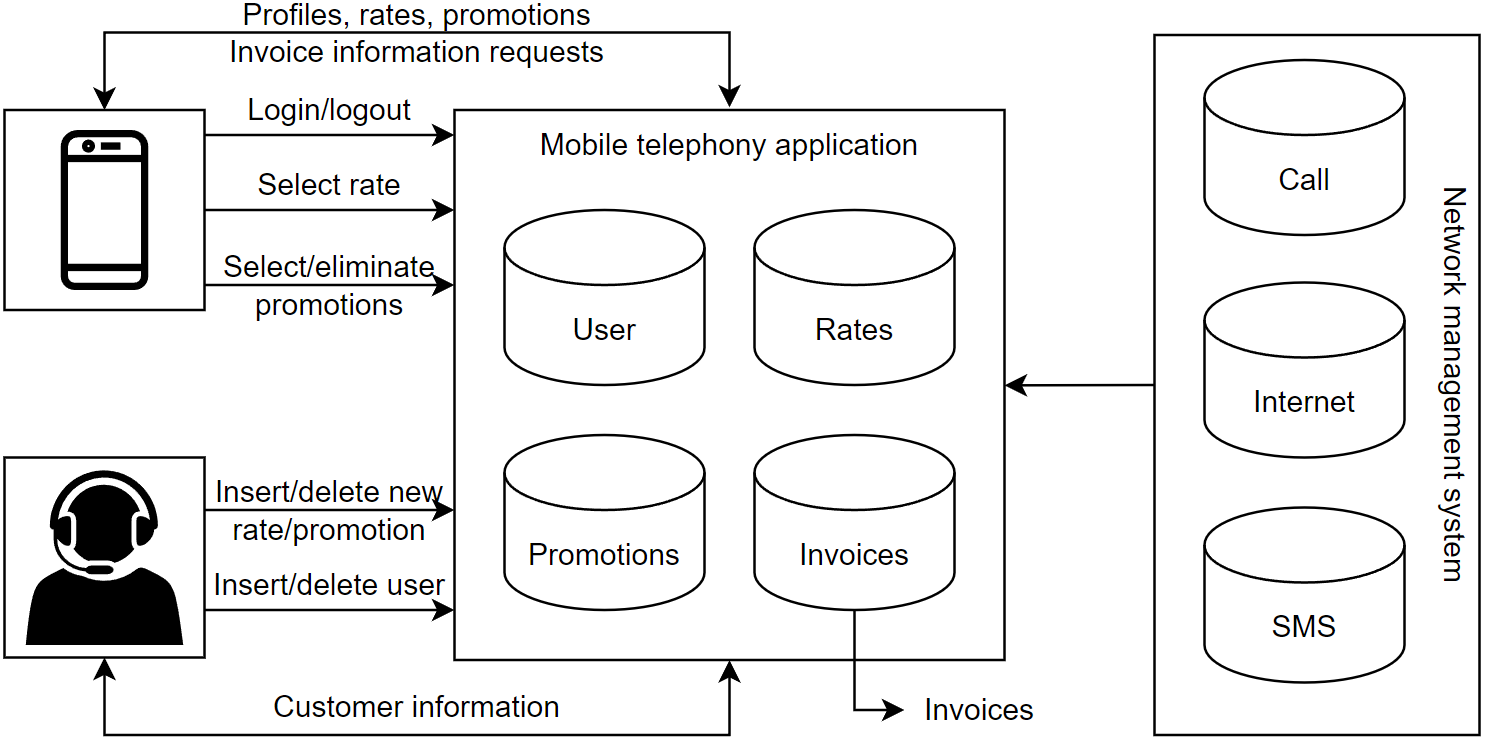
\includegraphics[width=0.75\linewidth]{images/fp.png}
    \end{figure}
    Now, let's consider each function type:
    \begin{itemize}
        \item \textit{Internal logic file}: the application retains data related to users, rates, promotions, and handles billing information, necessitating the generation of invoices.
            Each of these entities maintains a straightforward structure, comprising only a few fields. 
            Consequently, a simple weight of four is assigned to each, resulting in the ILF function point calculation as follows:
            \[\text{FP}_{\text{ILF}}=4 \cdot 7=28\]
        \item \textit{External interface file}: the application oversees communication with the network management system to obtain details regarding calls, SMS, and internet usage.
            There are three entities involved, each characterized by a straightforward structure.
            Consequently, a simple weight is chosen for all three entities:
            \[\text{FP}_{\text{EIF}}=3 \cdot 5=15\]
        \item \textit{External input}: the application engages with customers through various operations:
            \begin{itemize}
                \item Login/logout: these are simple operations, warranting the adoption of a simple weight for each:
                    \[\text{FP}=2 \cdot 3=6\]
                \item Select a rate: this operation involves two entities, the rate and the user, but it is still considered simple. 
                    Thus, the simple weight is applied:
                    \[\text{FP}=1 \cdot 3=3\]
                \item Select/eliminate a promotion: These operations involve three entities: the user, the rate, and the promotion. 
                    They are deemed to have medium complexity:
                    \[\text{FP}=2 \cdot 4=8\]
            \end{itemize}
            The application also interacts with company operators, enabling them to insert/delete information about a new rate or promotion and insert/delete information about a new user. 
            All four of these operations are considered to be of medium complexity:
            \[\text{FP}=4 \cdot 4=16\]
            In summary, the total external input function points can be calculated as:
            \[\text{FP}_{\text{EI}}=6+3+8+16=33\]
        \item \textit{External output}: the application enables customers to request details about their profiles, including lists of rates, promotions, and invoices tailored to them.
            Additionally, operators can visualize information for all customers. 
            In summary, there are five distinct external inquiries, each considered to have medium complexity:
            \[\text{FP}_{\text{EO}}=5 \cdot 4 = 20\]
        \item \textit{External inquiry}: the application facilitates the creation of invoices, representing a complex operation that necessitates gathering information from Internal Logic Files (ILFs) and External Interface Files (EIFs). 
            Therefore, the weight assigned for complex cases is applied:
            \[\text{FP}_{\text{EIN}}=1 \cdot 7 = 7\]
    \end{itemize}
    The cumulative number of function points is obtained by adding up all individual function points:
    \[\text{FP}_{\text{total}}=\text{FP}_{\text{ILF}}+\text{FP}_{\text{EIF}}+\text{FP}_{\text{EI}}+\text{FP}_{\text{EO}}+\text{FP}_{\text{EIN}}=28+15+33+20+7=103\]
\end{example}

\paragraph*{Summary}
The function point count is adjusted to account for the complexity of the project. 
Function points (FPs) can serve as a basis for estimating lines of code (LOC) by considering the average number of LOC per FP for a specific programming language:
\[\text{LOC}=\text{AVC}\cdot\text{number of function points}\]
In this formula, AVC is a language-specific factor that ranges from 200-300 for assembly language to 2-40 for a 4GL (fourth generation language).
It is crucial to note that FPs are highly subjective and contingent on the judgment of the estimator.